\documentclass{beamer}

\usetheme{Frankfurt}

\usepackage[utf8x]{inputenc}
\usepackage[ngerman]{babel}
\usepackage{subfigure}
\usepackage{caption}
\usepackage{listings}
\lstdefinelanguage{diff}
{
    morekeywords={+, -},
    sensitive=false,
    morecomment=[l]{//},
    morecomment=[s]{/*}{*/},
    morecomment=[l][\color{darkgreen}]{+},
    morecomment=[l][\color{red}]{-},
    morestring=[b]",
}


% draw
%\usepackage[rgb]{xcolor}
\definecolor{hublue}{rgb}{  0, .21, .42}
\definecolor{darkred}{rgb}{.5, 0, 0}
\definecolor{darkgreen}{cmyk}{0.7, 0, 1, 0.5}
\definecolor{darkblue}{rgb}{0, 0, .5}

\usepackage[lflt]{floatflt}

\setbeamertemplate{footline}{%
  \usebeamerfont{date in head/foot}
%  \insertshortauthor - \inserttitle{}\hfill
%  \usebeamertemplate{navigation symbols}\hfill
  \insertframenumber{}/\inserttotalframenumber}
\setbeamertemplate{sidebar right}{}


\title{SAFERTOUCH}
\institute[{Humboldt-Universität zu Berlin}]{\inst{}Humboldt-Universität zu Berlin}
\author[Magnus Müller \and Kai Warnicke \and Dominik Oepen]{Magnus Müller \and Kai Warnicke \and Dominik Oepen}
\date[16.02.2011]{16. Februar 2011}

\begin{document}
%%%%%%%%%%%% Teil Dominik
	\begin{frame}
		\titlepage
	\end{frame}

	\begin{frame}
		\frametitle{Overview}
		\tableofcontents
	\end{frame}	

  \section{Motivation}
	\begin{frame}
		\frametitle{Motivation}
		Touchscreen an Knoten um Anreize für Endnutzer zu schaffen sich einen EFWS-Knoten zu beschaffen.\\
		\begin{block}{Mögliche Einsatzgebiete}
			\begin{itemize}
				\item Heimautomatisierung
				\item Community-Dienste
				\item Location-based Services
			\end{itemize}
		\end{block}
	\end{frame}

	\section{Displaylink}
	
	\begin{frame}
		\frametitle{Displaylink}
		\begin{itemize}
			\item Chipsätze zur Konvertierung von USB nach DVI
			\item Serien DL-1x5 und DL-1x0
			\item Chipsätze kommt in Geräten unterschiedlicher Hersteller zum Einsatz 
        (Samsung, Nanovision)
		\end{itemize}	
	\end{frame}	

	\begin{frame}
		\frametitle{Mimo 720f}
		\begin{center}
			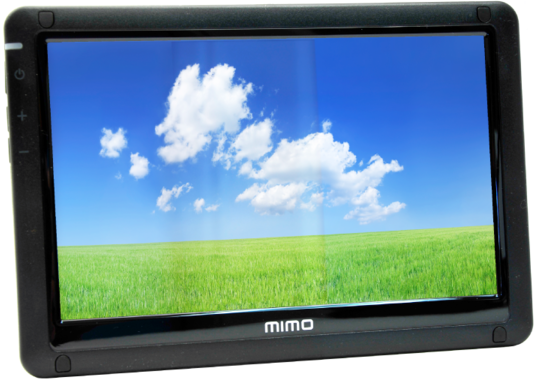
\includegraphics[scale=0.3]{img/mimo720f}
		\end{center}
		
		\begin{itemize}
			\item 7 Zoll Bildschirmdiagonale, Auflösung 800*480
			\item USB-Powered
			\item Touchscreen (e2i)
		\end{itemize}
	\end{frame}

  \subsection{Technische Details}
	\begin{frame}
		\frametitle{Displaylink}
		\begin{itemize}
			\item Stromchiffre zur Verschlüsselung der Daten (LFSR)
			\item Sehr effiziente Huffman-Codierung zur Kompression
			\item Reverse Enigeering durch Florian Echtler und Chris Hodges \footnote{Reverse-Engineering DisplayLink devices -- USB to DVI for hackers \url{http://events.ccc.de/congress/2009/Fahrplan/events/3353.en.html}}
			\item (Eingeschränkte) freie Treiber von Displaylink
			\item Offene Treiber aus der OSS Community
		\end{itemize}
	\end{frame}	
	

	\begin{frame}
		\frametitle{udlfb}
		\begin{itemize}
			\item Kerneltreiber um Displaylink Geräte als Framebuffer zu verwenden
			\item Andere Treiber existieren (z.B. X.org Treiber)
			\item Hervorgegangen aus libdlo (keine Huffmann-Codierung)
			\item Juni 2009 in Staging-Zweig des Kernel aufgenommen (2.6.31)
			\item November 2010 in Hauptzweig übernommen (2.6.37), erscheint ab 2.6.38 in
        mainline kernel.
		\end{itemize}
	\end{frame}	
			
	\begin{frame}
		\frametitle{Displaylink und OpenWRT}
    \begin{block}{Backfire}
        Der Standardkernel in Backfire (2.6.32.27) bringt bereits Unterstützung für udlfb
        mit. Wir benötigen aber einen aktuelleren Kernel, da sonst erstens der Touchscreen
        nicht funktioniert und zweitens udlfb in dieser Version nicht performant genug
        ist.
    \end{block}
    \begin{block}{Zwei Lösungsansätze}
				\begin{enumerate}
					\item Neueren Kernel in Backfire einbinden
					\item OpenWRT Developer-Branch nutzen
				\end{enumerate}
    \end{block}
	\end{frame}

%%%%%%%%%%%% Teil Magnus
  \section{Touchscreen}
	
	\begin{frame}
		\frametitle{Ansteuerung des Touchscreen}
		\begin{itemize}
			\item Getrennt von Framebuffer
			\item evtouch (X.org)
			\item Kerneltreiber e2i
			\item tslib zur Kalibrierung
		\end{itemize}
	\end{frame}	
	
	\section{Qt}
	
	\begin{frame}[containsverbatim, squeeze]
  %% Motivation fuer Verwendung von Qt
  \frametitle{Direkter Umgang mit Framebuffer ist mühsam}
		\begin{lstlisting}[language=C, basicstyle=\scriptsize]
struct fb_var_screeninfo screen;
ioctl(fd, FBIOGET_VSCREENINFO, &screeninfo);

int width = screeninfo.xres;
int height = screeninfo.yres;

__u16 *data = (__u16 *) mmap (0, width*height*2, 
                PROT_READ|PROT_WRITE, MAP_SHARED, fd, 0);

for (int row = 0; row < height; row++) {
    for (int column = 0; column< width; column++) {
        data[column+row*width] = 0xe111;
    }
}

int coords[4] {0, 0, screen.xres_virtual, screen.yres_virtual};

if (ioctl (fd, DL_IOCTL_BLIT, &coords) == -21) 
    fprintf (stderr, "Error on ioctl call.\n");

munmap (data, width*height);
		\end{lstlisting}
	\end{frame}	
	
	\begin{frame}
		\frametitle{Qt}
		\begin{floatingfigure}[l]{1.75cm}
			
\includegraphics[scale=0.3]{img/qt-logo}
		\end{floatingfigure}
		\begin{quote}
		Qt is a cross-platform application  and UI framework used by hundreds of thousands of developers worldwide looking to create amazing user experiences  on Windows, Mac, Linux/X11, embedded Linux, Windows CE , Windows Mobile, Symbian  and Maemo devices.
		\end{quote}
    \begin{itemize}
      \item Intuitive C++ class library
      \item Portability across desktop and embedded operating systems
      \item Integrated development tools with cross-platform IDE
      \item High runtime performance and small footprint on embedded
    \end{itemize}
	\end{frame}	
	
	\begin{frame}
		\frametitle{Qt und Displaylink}
    \begin{block}{Framebuffer \& Qt}
      \begin{itemize}
        \item Qt enthält Framebufferunterstützung (linuxfb und directfb)
        \item Funktioniert nicht mit udlfb
        \item Grund: Fehlender ioctl zur Aktualisierung des Bildschirminhalts
      \end{itemize}
    \end{block}
    \begin{block}{Touchscreen \& Qt}
        \begin{itemize}
          \item Qt enthält Touchscreenunterstützung (LinuxInput, tslib, \ldots)
          \item Funktioniert nicht out-of-the-box mit e2i
          \item Grund: Kalibrierung von tslib ist nötig und Umgebungsvariablen müssen gesetzt
            werden.
        \end{itemize}
    \end{block}
	\end{frame}
	
  \subsection{Framebuffer}
	\begin{frame}[containsverbatim, allowframebreaks, squeeze]
		\frametitle{Qt patch für udlfb}
		\begin{lstlisting}[language=diff, basicstyle=\tiny]
--- qscreenlinuxfb_qws.cpp.org	2011-02-04 16:11:34.000000000 +0100
+++ qscreenlinuxfb_qws.cpp2011-02-04 16:20:39.741035002 +0100
@@ -337,7 +337,12 @@
         return false;
     }
 
-    d_ptr->driverType = strcmp(finfo.id, "8TRACKFB") ? GenericDriver : EInk8Track;
+    if (!strcmp(finfo.id, "8TRACKFB"))
+        d_ptr->driverType = EInk8Track;
+    else if (!strcmp(finfo.id, "udlfb"))
+        d_ptr->driverType = UDLFB;
+    else
+        d_ptr->driverType = GenericDriver;
 
     if (finfo.type == FB_TYPE_VGA_PLANES) {
         qWarning("VGA16 video mode not supported");
@@ -1252,6 +1257,9 @@
             ioctl(d_ptr->fd, 0x46a2, 1);
         else
             ioctl(d_ptr->fd, 0x46a2, 0);
+    } else if (d_ptr->driverType == UDLFB) {
+        int coords[4] = {r.left(), r.top(), r.right(), r.bottom()};
+        ioctl(d_ptr->fd, 0xAA, &coords);
     }
 }



 
--- qscreenlinuxfb_qws.h.org	2011-02-04 16:12:27.000000000 +0100
+++ qscreenlinuxfb_qws.h	2011-02-04 16:23:11.241035001 +0100
@@ -88,7 +88,7 @@
 
     virtual bool useOffscreen();
 
-    enum DriverTypes { GenericDriver, EInk8Track };
+    enum DriverTypes { GenericDriver, EInk8Track,  UDLFB};
 
     virtual void disconnect();
     virtual void shutdownDevice();	
		\end{lstlisting}
	\end{frame}

  \subsection{Touchscreen}
	\begin{frame}[containsverbatim, allowframebreaks]
    \frametitle{Umgang mit tslib}
    \begin{block}{Umgebungsvariablen}
      \begin{lstlisting}[language=Bash]
export TSLIB_CONSOLEDEVICE=none
export TSLIB_FBDEVICE=/dev/fb0
export TSLIB_TSDEVICE=/dev/input/event0
export TSLIB_CALIBFILE=/etc/pointercal
export TSLIB_CONFFILE=/etc/ts.conf
export TSLIB_PLUGINDIR=/usr/lib/ts
export QWS_MOUSE_PROTO=tslib:/dev/input/event0
      \end{lstlisting}
    \end{block}
    \begin{block}{Kalibrierung}
      \begin{lstlisting}[language=Bash]
        tests/ts_calibrate
      \end{lstlisting}
    \end{block}
    \begin{block}{Preload}
      \begin{lstlisting}[language=Bash]
LD_PRELOAD=/usr/lib/libts.so executable -qws
      \end{lstlisting}
    \end{block}
  \end{frame}

\end{document}
